\documentclass[11pt,a4paper,oldfontcommands,openany]{memoir}
\usepackage[utf8]{inputenc}
\usepackage[T1]{fontenc}
\usepackage{microtype}
\usepackage[dvips]{graphicx}
\usepackage[dvipsnames]{xcolor}
\usepackage{times}
\usepackage{amsmath}
\usepackage{amsthm}
\usepackage{syntax}
\usepackage{multicol}
\usepackage[]{algorithm2e}
\usepackage{xcolor}
\usepackage{tabularx}
%\usepackage{algorithm}

\usepackage[
breaklinks=true,colorlinks=true,
%linkcolor=blue,urlcolor=blue,citecolor=blue,% PDF VIEW
linkcolor=black,urlcolor=black,citecolor=black,% PRINT
bookmarks=true,bookmarksopenlevel=2]{hyperref}

\usepackage{geometry}%top=25mm,bottom=25mm
% PDF VIEW
 \geometry{total={210mm,297mm},
 left=25mm,right=25mm,
 bindingoffset=0mm, top=24mm,bottom=24mm}
% PRINT
%\geometry{total={210mm,297mm},
%left=20mm,right=20mm,
%bindingoffset=10mm, top=24mm,bottom=24mm} 

\OnehalfSpacing
%\linespread{1.3}

%%% CHAPTER'S STYLE
\chapterstyle{bianchi}
%\chapterstyle{ger}
%\chapterstyle{madsen}
%\chapterstyle{ell}
%%% STYLE OF SECTIONS, SUBSECTIONS, AND SUBSUBSECTIONS
\setsecheadstyle{\Large\bfseries\sffamily\raggedright}
\setsubsecheadstyle{\large\bfseries\sffamily\raggedright}
\setsubsubsecheadstyle{\bfseries\sffamily\raggedright}


%%% STYLE OF PAGES NUMBERING
%\pagestyle{companion}\nouppercaseheads 
%\pagestyle{headings}
%\pagestyle{Ruled}
\pagestyle{plain}
\makepagestyle{plain}
\makeevenfoot{plain}{\thepage}{}{}
\makeoddfoot{plain}{}{}{\thepage}
\makeevenhead{plain}{}{}{}
\makeoddhead{plain}{}{}{}


\maxsecnumdepth{subsection} % chapters, sections, and subsections are numbered
\maxtocdepth{subsection} % chapters, sections, and subsections are in the Table of Contents

\newtheorem*{theorem}{Theorem}
\newtheorem*{definition}{Definition}
\newtheorem*{property}{Property}
\newtheorem*{lemma}{Lemma}

%%%---%%%---%%%---%%%---%%%---%%%---%%%---%%%---%%%---%%%---%%%---%%%---%%%

\begin{document}
\pagenumbering{gobble}
%%%---%%%---%%%---%%%---%%%---%%%---%%%---%%%---%%%---%%%---%%%---%%%---%%%
%   TITLEPAGE
%
%   due to variety of titlepage schemes it is probably better to make titlepage manually
%
%%%---%%%---%%%---%%%---%%%---%%%---%%%---%%%---%%%---%%%---%%%---%%%---%%%
\thispagestyle{empty}

{%%%
\sffamily
\centering
\Large

~\vspace{\fill}

{\huge 
Generalization of counterexamples for inductive invariant synthesis
}

\vspace{2.5cm}

{\LARGE
Mickaël LAURENT
}

\vspace{3.5cm}

Carnegie Mellon University\\
Ecole Normale Supérieure Paris-Saclay

\vspace{3.5cm}

Supervisor: Bryan PARNO

\vspace{\fill}

March-July 2018

%%%
}%%%

\clearpage%\cleardoublepage
%%%---%%%---%%%---%%%---%%%---%%%---%%%---%%%---%%%---%%%---%%%---%%%---%%%
%%%---%%%---%%%---%%%---%%%---%%%---%%%---%%%---%%%---%%%---%%%---%%%---%%%

\tableofcontents*

\clearpage

%%%---%%%---%%%---%%%---%%%---%%%---%%%---%%%---%%%---%%%---%%%---%%%---%%%
%%%---%%%---%%%---%%%---%%%---%%%---%%%---%%%---%%%---%%%---%%%---%%%---%%%
\pagenumbering{arabic}
\setcounter{page}{1}
\chapter{Presentation of IVy}

    \section{Context}

    As distributed programs become more and more widespread, their verification is a major challenge.
    The general purpose of my internship is to make the certification of those programs easier, by providing new methods and semi-automated tools that will assist the user in this process.
    Certifying a program consists in writing some specifications (in our case, some safety properties), and then proving than the program satisfy them.
    Several languages and tools already exist for that:

    \begin{itemize}
        \item Proof-assistants (Coq, F*, etc.):
        Powerful logics can be used for the specification,
        however the user has to manually write the proof (in a interactive way).
        \item SMT-solver based tools (dafny, F*, etc.):
        Logics and constructions are often restricted, but specifications can automatically be checked using a SMT-solver.
        Most of time, this process is undecidable,
        so there are 3 possible outputs:
        \begin{itemize}
            \item Yes, the program matches the specifications
            \item No, the program doesn't match the specifications (sometimes a counterexample can be provided)
            \item I don't know whether the program matches the specifications or not.
        \end{itemize}
        When this last case occurs, the user has to reformulate the specifications differently or to explicitely write some intermediate properties (like inductive invariants)
        in order to help the SMT-solver.
    \end{itemize}

    IVy\cite{Padon:2016:ISV:2908080.2908118} is a language and a set of tools that allows the user to certify its program using a SMT-solver based approach.
    However, unlike most of its concurrents, IVy restricts the language and the logic used for specifications
    in order to be able to check the program in a decidable way.

    This approach has many advantages:
    \begin{itemize}
        \item Once the program is written and specified in an accepted logic, it can be checked more easily:
        the checker can always decide whether the program matches the invariants or not, and give a counterexample if it does not.
        \item It does not rely on any heuristic/specificity of the SMT-solver used.
        When a program cannot be checked, a precise reason is provided.
        \item A program can be checked with any version of any SMT-solver (because it does not depend on any heuristic).
    \end{itemize}
    
    The main disadvantage is that the user is forced to specify its program in a decidable fragment of first order logic:
    it can force him to rethink the architecture of its code, to fragment its code by creating intermediate abstract modules,
    to add some `ghost' variables, etc.

    \section{The RML language}

    IVy is inspired by a modeling language called RML (Relational Modeling Language)\cite{Padon:2016:ISV:2908080.2908118}. It is restricted such that some decidability properties are guaranteed (see section 1.4).
    A RML program is composed of:
    \begin{itemize}
        \item Some uninterpreted types called `sorts'. `Uninterpreted' means that these types are not interpreted in any existing theory like arithmetic:
        they are just set of values without any specific structure, though we can add axioms to our system (see below).
        A sort has an unbounded number of elements.
        Some enumerated types can also be defined (= types with fixed finite number of elements).
        \item Some variables, relations and functions over these types (a variable can be considered like a function of arity 0, and a relation can be considered as a function
        which returns a boolean). These elements are mutable (their valuation can be modified by the transitions described below).
        \item Some axioms over these types, variables, functions and relations. Axioms are \(\exists^*\forall^*\) formulas (\( \phi_{EA} \) in the grammar below).
        \item Some transitions that we call `actions'. An action is characterized by a name and a \(statement\) (see the grammar below).
        \item A special `init' action that is only executed once at the beginning (before any other action).
        \item A set of safety properties, that are first order formulas that should be satisfied after the execution of any action in a valid run (starting with the `init' action).
        Only a restricted fragment of first order logic can be used, for decidability reasons (see sections 1.3 and 1.4).
    \end{itemize}

    The transitions can be written using the following grammar:
    \begin{multicols}{2}
        \begin{grammar}

            <statement> ::= skip
            \alt abort
            \alt \textbf{r}(\(\bar{x}\)) := \( \phi_{QF}(\bar{x}) \)
            \alt \textbf{f}(\(\bar{x}\)) := \( t(\bar{x}) \)
            \alt \textbf{v} := \( * \)
            \alt assume \( \phi_{EA} \)
            \alt \( statement \) ; \( statement \)
            \alt \( statement \) | \( statement \)
            
        \end{grammar}

        \columnbreak

        \begin{grammar}

            <t> ::= \(x\)
            \alt \textbf{v}
            \alt \textbf{f}(\(t,\ldots t\))
            \alt ite(\( \phi_{QF},t,t\))

            <\( \phi_{QF} \)> ::= \textbf{r}(\(t,\ldots t\))
            \alt \( t = t \)
            \alt \( \phi_{QF} \land \phi_{QF} \) \quad | \quad \( \phi_{QF} \lor \phi_{QF} \) \quad | \quad \( \neg \phi_{QF} \)
            
            <\( \phi_{EA} \)> ::= \( \exists x_1,\ldots,x_n \forall x_{n+1},\ldots,x_{n+m} \phi_{QF} \)

        \end{grammar}
    \end{multicols}

    The semantic of terms and formulas is as usual. The semantic of statements will be described later in the section 1.4.

    One important thing to note is that types can only be uninterpreted sorts or enumerated types (like booleans).
    It means that the structure of these types and the operations over them are only constrained by the axioms of the RML program,
    and the form of these axioms is quite restrictive.
    In particular, we can't define arithmetic operations (see section 1.3).

    Also, unlike some other languages like F*, we can't have refinement types or dependent types.
    As a consequence, we can't encode any property in the types.
    Instead, the specifications of the program are expressed with assertions (that can be built with the primitives `|', `assume' and `abort')
    and safety properties.

    \section{Decidable logics}

    In this section, we will describe the Bernays-Schönfinkel class of formulas. It is a decidable fragment of the first order logic that is used in RML.
    We will refer to it as EPR (for Effectively Propositional) because this logic can be effectively translated into propositional logic (see the subsection 1.3.2).

        \subsection{The Bernays-Schönfinkel class (EPR)}

        The Bernays-Schönfinkel class is the set of first-order formulas such that:
        \begin{itemize}
            \item Under the prenex normal form, they have an \(\exists^*\forall^*\) quantifier prefix
            (a formula in prenex normal form is composed of a string of quantifiers called the prefix, followed by a quantifier-free part).
            \item They do not use any function symbol (only a finite number of constants and relations).
        \end{itemize}

        For instance, the following formulas define a total relation order and are in the Bernays-Schönfinkel class:
        \begin{align*}
            \forall x. \ R(x,x) &\quad\text{(reflexivity of R)}\\
            \forall x,y,z. \ R(x,y) \land R(y,z) \rightarrow R(x,z) &\quad\text{(transitivity of R)}\\
            \forall x,y. \ R(x,y) \land R(y,x) \rightarrow x=y &\quad\text{(antisymetry of R)}\\
            \forall x,y. \ R(x,y) \lor R(y,x) &\quad\text{(totality of R)}
        \end{align*}

        \subsection{Deciding the satisfiability}

        We want to decide whether an EPR formula is satisfiable or not. Let's consider for instance the following formula:
        \begin{align*}
            F: \exists x. \forall y. \ R(y,y) \land \neg R(x,y)
        \end{align*}

        This formula is not satisfiable, because for any value of \(x\), the formula \(R(y,y) \land \neg R(x,y)\) is false when we take \(y=x\).
        However, there is infinitely many possible interpretations for the relation \(R\) (because the set of possible values for \(x\) and \(y\) is not bounded).
        So how to decide the satisfiabilty of such formulas?

        First, we can get rid of the existential quantifier by introducing a new constant \(A\):
        \begin{align*}
            \forall y. \ R(y,y) \land \neg R(A,y)
        \end{align*}

        This is called the skolem normal form of \(F\).
        In the general case, we can eliminate any existential quantifier of a formula in prenex normal form by introducing a new function
        that depends on all previously declared universally quantified variables. This process is called `skolemization' and it preserves the satisfiability of the formula.

        \begin{property}[Skolemization]
            Let \(F\) be a formula and \(F'\) be the formula obtained after solemization of \(F\). Then \(F\) is satisfiable iff \(F'\) is satisfiable.
        \end{property}

        Now, we want to restrict the domain of the possible interpretations in order to be able to decide the satisfiability of our formula.

        \begin{definition}[Herbrand domain]
            The Herbrand domain of a formula is the set of every term that can be written with constants and functions symbols that are used in the formula
            (if there is no constant symbol in the formula, a new fresh constant symbol can be used).
        \end{definition}

        Our formula has a unique constant \(A\) and no function symbol (only a relation symbol), so its Herbrand domain is the following:
        \( \{A\} \). More generally, we have the following property:
        
        \begin{property}
        The Herbrand domain of an EPR formula is finite.
        \end{property}

        Thus, we can decide whether or not our formula is satisfiable by an interpretation over it's Herbrand domain.
        For that, we just have to test every interpretation of \(R\) over the domain \( \{A\} \):

        \begin{itemize}
            \item With \(R(A,A)=\text{false}\): \(\forall y. \ R(y,y) \land \neg R(A,y)\) is false (with \( y \in \{A\} \))
            \item With \(R(A,A)=\text{true}\): \(\forall y. \ R(y,y) \land \neg R(A,y)\) is false (with \( y \in \{A\} \))
        \end{itemize}

        So our formula is not satisfiable by any interpretation over it's Herbrand domain.

        Finally, by applying the following theorem, we can conclude that our formula is not satisfiable by any interpretation (over any domain):
        \begin{theorem}[Herbrand]
            An universally quantified first-order formula \(F\) is satisfiable iff it is satisfied by an interpretation over it's Herbrand domain.
        \end{theorem}

        This process can be used to decide the satisfiability of any EPR formula. Moreover, when a formula is satisfiable,
        it gives us an interpretation over the Herbrand domain that satisfy the formula.
        The Herbrand domain being finite, we have the following property:

        \begin{property}[Finite model property]
            Every satisfiable EPR formula has a finite model.
        \end{property}

        \subsection{EPR with types}

        In RML, relations, functions and constants (that are preferably called `variables' since they are mutable) have types.
        In particular, the arguments and the output of a function have types.
        We can easily add these typing constraints to the logical symbols we used in the previous subsection.
        Moreover, it allows us to extend the domain of EPR formulas by still keeping a finite Herbrand domain.

        Indeed, we can allow function symbols and \(\forall\exists\) quantifier alternation as long as,
        once the formula is skolemized, we have the following property (we say that function symbols are \textbf{stratified}):
        there exists a strict order `<' over the unbounded sorts such that,
        for every function symbol \( f: t_1,\ldots,t_n \to t \), we have \( t_i < t \) for all \(i \in [1..n]\) such that \(t_i\) and \(t\)
        are unbounded sorts. 

        However, the EPR fragment can still be too restrictive: for instance, we can't introduce linear arithmetic using only EPR axioms.
        Indeed, the standard way to define integers is to introduce a successor function symbol, which is not allowed because it can't be stratified.
        More generally, we can't characterize any infinite set with only EPR axioms: it would contradict the finite model property.

        Actually, some strict extensions of EPR are still decidable, for instance the Finite Almost Uninterpreted fragment\cite{Taube:2018:MDD:3192366.3192414} which allows
        some basic linear arithmetic. However, we will not use such extensions in this report because it breaks the finite model property.

        %\subsection{Extensions of EPR}

        %Some strict extensions of EPR are still decidable.
        %In particular, SMT-solvers like Z3 are able to decide the Finite Almost Uninterpreted (FAU) fragment of first order logic,
        %which add to EPR some usual interpreted symbols of Linear Arithmetic (integer constants, `+', `\( \leq \)') under some additional constraints.
        %In this report, we will not use such extension of EPR, because it breaks the finite model property.
    
    \section{Checking a RML program}

    \begin{definition}[Structure \& State]
        For a given RML program, a structure (or interpretation) is a pair \(((D_s)_{s\in \text{sorts}}, (I_s)_{s\in \text{symbols}})\) where:
        \begin{itemize}
            \item For all \(s \in \text{sorts}\), \(D_s\) is a finite domain associated to the sort \(s\).
            \item For all \(s \in \text{symbols}\) (variable, function or relation), \(I_s\) is a valuation for the symbol \(s\) (using the domains \((D_s)_{s\in \text{sorts}}\)).
        \end{itemize}
        A state is a structure that satisfy every axiom of the RML program.
    \end{definition}

    In order to certify that a RML program never abort abnormally and satisfy its safety properties, we must provide IVy with an invariant \(I\) such that:
    \begin{enumerate}
        \item \(I\) is initially satisfied (after any execution of the `init' action starting from any state).
        \item Any state satisfying \(I\) also satisfy all the safety properties.
        \item \(I\) is \textbf{inductive}, that is: from any state satisfying \(I\), any execution of one step (= one action) will not fail and
        will lead to a new state that also satisfy \(I\). 
    \end{enumerate}

    To formalize these properties, we introduce the notion of weakest precondition \(wp\):
    \begin{definition}[Weakest precondition]
        For any statement \(S\) and formula \(Q\), the weakest precondition of \(Q\) by \(S\) (noted \(wp(S,Q)\)) is the weakest formula \(P\) such that
        every execution of \(S\) starting from a state satisfying \(P\) will lead to a state that satisfies \(Q\).
    \end{definition}

    Weakest preconditions can be computed as follows\cite{Padon:2016:ISV:2908080.2908118}:\\

    \begin{tabular}{|l|l|l|}
        \hline
        Statement & Semantic & \( wp(\text{statement},Q) \) \\
        \hline
        skip & Do nothing & \(Q\) \\
        abort & Terminate abnormally (fail) & false \\
        \textbf{r}(\(\bar{x}\)) := \( \phi_{QF}(\bar{x}) \) & Quantifier-free update of relation \textbf{r} & \((A_r \rightarrow Q) [\phi_{QF}(\bar{s})\ /\ \text{\textbf{r}}(\bar{s})]\) \\
        \textbf{f}(\(\bar{x}\)) := \( t(\bar{x}) \) & Update of function \textbf{f} to term \( t(\bar{x}) \) & \((A_f \rightarrow Q) [t(\bar{s})\ /\ \text{\textbf{f}}(\bar{s})]\) \\
        \textbf{v} := \( * \) & Non-deterministic assignment of variable \textbf{v} & \(\forall x. (A_v \rightarrow Q) [x\ /\ \text{\textbf{v}}]\)\\
        assume \( \phi_{EA} \) & Assume a \( \exists^*\forall^* \) formula holds & \( \phi_{EA} \rightarrow Q \) \\
        \( S_1 \) ; \( S_2 \) & Sequential composition & \( wp(S_1, wp(S_2, Q)) \) \\
        \( S_1 \) | \( S_2 \) & Non-deterministic choice & \( wp(S_1, Q) \land wp(S_2, Q) \) \\
        \hline
    \end{tabular}\\ \\
    \( \phi(\beta,\alpha) \) denotes \(\phi\) with occurences of \(\alpha\) substituted by \(\beta\), and \(A_s\) denotes the axioms of the RML program
    that involve the symbol \(s\).\\
    \\
    Now, the properties above can be rewritten using weakest preconditions:
    \begin{enumerate}
        \item \(A \Rightarrow wp(\text{init},I)\)
        \item For any safety property \(P\), \(I \Rightarrow P\)
        \item \(A \land I \Rightarrow wp(\text{action}_1|\ldots|\text{action}_n,I)\)
    \end{enumerate}

    \begin{lemma}
        Let \(S\) be a RML statement and \(Q\) a \(\forall^*\exists^*\) formula (= a formula whose normal prenex form has a \(\forall^*\exists^*\) prefix followed by a quantifier-free part), then \(wp(S,Q)\) is also a \(\forall^*\exists^*\) formula.
    \end{lemma}

    This lemma can easily be proved by induction on \(S\) (we remind that axioms \(A\) are \(\exists^*\forall^*\) formulas).
    
    Moreover, according to the section 1.3, satisfiability of \(\exists^*\forall^*\) formulas can be checked if function symbols are stratified.
    We can deduce the following theorem:

    \begin{theorem}[]
        Let \(S\) be a RML statement, \(P\) a \(\exists^*\forall^*\) formula and \(Q\) a \(\forall^*\exists^*\) formula.
        Then, if all function symbols are stratified, checking the validity of the three formulas above is decidable
        (it can be done by checking the satisfiability of their negation).
    \end{theorem}

    In particular, checking whether a formula with no quantifier alternation satisfies these three properties is decidable.
    In practice, since satisfiability of some formulas with \( \forall\exists \) quantifier alternation can still be decidable,
    some invariants with quantifier alternation are allowed in RML. However, if an invariant can't be checked in a decidable way, IVy will reject it
    and will indicate to the user the faulty functions or quantifier alternations.

    \section{Challenges and current research}

    As we have just seen, some inductive invariants can be checked in a decidable way.
    However, it does not mean that they can be automatically produced.

    Indeed, when writing a protocol using IVy, the two main challenges are:
    \begin{itemize}
        \item The implementation and specification of programs, in accordance with the restrictions of RML
        (stratification of functions, restriction on formulas, no recursion... though some additional primitives can be added to RML).
        A lot of research is in progress in order to help the user to make such programs. In particular, two majors methods are
        studied: the fragmentation of the code into many independent modules that can use different fragments of the first-order logic\cite{Taube:2018:MDD:3192366.3192414},
        and the insertion of some mutable `ghost' relations in the program that aim to capture the values of some formulas\cite{Padon:2017:PME:3152284.3140568}.
        
        \item The finding of an inductive invariant (once the program is implemented and specified). As we will see in the next part,
        IVy can help the user to find an inductive invariant by providing a counterexample if the current invariant is not inductive.
        From this counterexample, a new conjecture can be automatically generated in order to strengthen the current invariant.
        My work has consisted in improving this synthesis.
    \end{itemize}

    Some other challenges are also studied, like the verification of liveness properties\cite{Padon:2017:RLS:3177123.3158114}.

%\chapter{Research directions}
%    \section{Make code EPR}
%        \subsection{Fragmentation}
%        \subsection{Adding relations}
%    \section{Adding typing}
%    \section{Invariant Synthesis}

\chapter{Invariant synthesis}

    \section{Introduction}

    The synthesis of an inductive invariant is a common problem in verification, and even with the restrictions of RML, it is still undecidable (though it can be decidable for some very restricted classes of invariants)\cite{Padon:2016:DII:2914770.2837640}.
    Nevertheless, even an partial resolution of this problem can still be very helpful for the user.

    In the context of RML programs, most of invariants can be expressed with universal formulas (\(\forall^*\)), but sometimes a \(\forall^*\exists^*\) formula can be required (under some restrictions in order
    to stay in a decidable fragment of logic). Thus, we will restrain our search to these two types of invariant.
    In particular, when possible, we will try to synthetize universal invariants because they are easier to generate and will never cause any decidability issue.
    
    As described in this article\cite{Karbyshev:2017:PIU:3065931.3022187}, a common way to find an inductive invariant is to start from the safety properties of the program
    and try to sthrengthen them by adding new invariants (using one of the methods described in the next sections) until the resulting set of invariants form an inductive invariant
    (thereafter, we will use the terms `invariant' or `set of invariants' indistinguishably: a set of invariants can be seen as a single invariant that is the conjunction of all the invariants of the set).
    This iterative process may not terminate, but it offers to the user an interactive way to find an inductive invariant:
    if the current invariant is not inductive, a new conjecture is proposed to the user (in order to sthrengthen the current invariant).
    If this conjecture is simple enough, the user can understand it and adjust it as he wants (making it stronger, resolving decidabilities issues, etc.), and we repeat this process.

    Thus, the problem we want to solve is the following:
    given an invariant that is not inductive, we want to strenghten it by generating a new (correct) invariant as strong as possible, if possible without breaking the decidability of the system.
    To be correct, an invariant must be satisfied by every state that can be obtained with a valid execution (beginning with the `init' action).
    The following criteria can be used to evaluate an algorithm that tries to solve this problem:
    \begin{enumerate}
        \item \textbf{Reliability}: Can the algorithm fail, not terminate or generate incorrect invariants?
        \item \textbf{Decidability}: Is the new set of invariants generated checkable in a decidable way (in our case, we want it to be EPR)?
        \item \textbf{Efficiency}: How strong is the new invariant generated? Is it easily understandable by the user (in order to be adjusted if needed)?
    \end{enumerate}

    \section{Weakest precondition as a new invariant}

    One possible way to sthrengthen an invariant \(I\) is to make the conjunction with its weakest precondition \(wp(\text{action}_1|\ldots|\text{action}_n,I)\).
    If the initial invariant is not inductive, the result will be strictly stronger.

    Let's evaluate this method with the criteria above.\\
    
    \textbf{Reliability}: This method always terminates and never fails. Moreover, it produces correct invariants. Here is a proof:

    We assume that the initial invariant \(I\) is correct. Let \(P = wp(\text{action}_1|\ldots|\text{action}_n,I)\).

    By contradiction, let's suppose that we have a state \(S\), issued from a valid execution \(E\), that doesn't satisfy \(P\).
    Two cases are possible:
    \begin{itemize}
        \item There exists an execution \(E'\) of one step (= one action) starting in \(S\) such that the resulting state \(S'\) doesn't satisfy the initial invariant.
        \(E\) followed by \(E'\) is a valid execution that results in the state \(S'\). As \(S'\) doesn't satisfy \(I\), we have a contradiction.
        \item Every possible execution of one step starting in \(S\) will result in a state that satisfy \(I\).
        In this case, we can generate a precondition for our initial invariant that is stricly weaker than \(P\):
        let \(F\) be a formula that fully characterize \(S\) modulo isomorphism (it can be done by constraining the cardinality of the domains and the valuations of the different symbols in these domains),
        then \(P \lor F\) is still a precondition for \(I\) and is strictly weaker than \(P\) (contradiction). 
    \end{itemize}

    So \(P\) is a correct invariant.\\

    \textbf{Decidability}: Even if the initial invariant is EPR, the weakest precondition is not guaranteed to be EPR.
    Indeed, when computing the weakest precondition, stratification can be broken on several cases: assumptions, non-deterministic operations, etc.

    Nevertheless, we can have the guarantee that the weakest precondition is EPR by adding these restrictions:
    \begin{itemize}
        \item All function symbols used must be stratified.
        \item The initial invariant must be universally quantified.
        \item Assumptions must be existentially quantified.
        \item Axioms that involve a mutable variable, function or relation must be existentially quantified.
    \end{itemize}
    We can easily verify that under these conditions, the weakest precondition will be an universally quantified formula
    and thus will be EPR. However, these conditions are very restrictive and so they can't be reasonably imposed.
    \\

    \textbf{Efficiency}: Weakest preconditions aim to be `weakest', while we want an invariant as strong and simple as possible.
    They are usually very long, even after simplification (they can grow exponentially).
    Moreover, they are not focused on one aspect in particular (they mix many different elements together), and so they are even more complicated
    to understand. 

    \section{Naive counterexample generalization}

    In order to produce simpler invariants, we can focus our search on a concrete counterexample.

    \begin{definition}[Counterexample]
    A counterexample is a pair \( (S,E) \) where \(S\) is a state that satisfies the current invariant and \(E\) is a deterministic statement that describes the execution of an action,
    starting from \(S\) and leading to a new state \(S'\) that doesn't satisfy the current invariant.
    \end{definition}
    Thanks to the finite model property of EPR (section 1.3.2), we are always able to find a finite counterexample when the current invariant is not inductive
    (section 1.4 explains how to check the inductiveness of an invariant).

    Let \( (S,E) \) be a finite counterexample.

    \begin{definition}
        Let \(S\) be a state, then \(constr(S)\) is the set of all constraints of the following forms that are satisfied by \(S\):
        \begin{itemize}
            \item \(symbol(concrete\_value_1,\ldots,concrete\_value_n) = concrete\_value\) with `\(symbol\)' refering to any variable, function or relation of \(S\) and `concrete values'
            being elements of the domains of \(S\)
            \item \(concrete\_value_1 \neq concrete\_value_2\) (where `\(concrete\_value_1\)' and `\(concrete\_value_2\)' have the same type)
        \end{itemize}
    \end{definition}

    We can generate a formula as follows:
    \begin{enumerate}
        \item We associate a fresh variable \( X_v \) to each concrete value \(v\) in \(S\).
        \item In each constraint of \(constr(S)\), we replace each concrete value \(v\) by \( X_v \).
        \item We make the conjunction of all these constraints and we quantify existentially on each \(X_v\). Optionaly, we can simplify the resulting formula to get rid of some variables.
    \end{enumerate}
    
    The resulting formula \(F\) is an existentially quantified formula that characterizes all the structures containing a substructure that is isomorphic to the structure of the counterexample.
    In order to prevent this counterexample from happening again, we just have to negate \(F\) (it will become universally quantified) and add it to the current set of invariants.

    This technique always generate an universal invariant, and so there is no decidability issue (if the function symbols are stratified).
    However, there are three major issues:
    \begin{itemize}
        \item As we will see in the next section, the new invariant generated is not always correct.
        \item The formula generated can be very long, because it contains all the constraints characterizing our counterexample.
        \item The formula generated is very specific: it will not prevent other \textit{similar} counterexamples from happening, as long as
        at least one constraint differs, even if this difference has no impact.
    \end{itemize}

    \section{A problematic example with non-monotonicity}

    Let's try the naive counterexample generalization on this IVy code:\\

    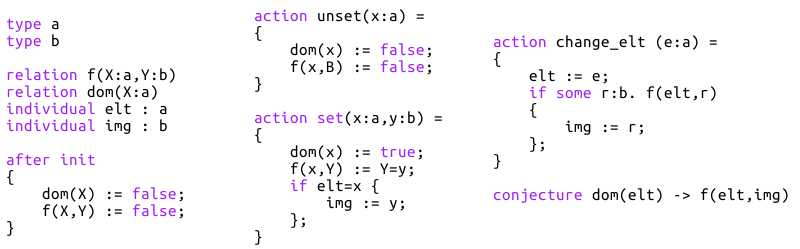
\includegraphics[width=15cm]{NonMonotonicExLarge}
    \\
    The keyword \textit{individual} is used to declare a variable, and the construction \textit{if some \(x\). \(\phi(x)\) \{ statement \}}
    assigns to the variable \(x\) a value \(v\) such that \(\phi(v)\) is true and executes \textit{statement}. If no such value \(v\) exists,
    \textit{statement} is not executed.

    Basically, this example defines the following:
    \begin{itemize}
        \item Two uninterpreted sorts \(a\) and \(b\).
        \item A relation \(f\) from \(a\) to \(b\) that will represent a partial function, and \(dom\) its domain. It might look curious to not directly define a function instead,
        but it can sometimes be useful for decidability reasons, as functions are subject to stratification constraints.
        \item A variable \(elt\) in \(a\) and a variable \(img\) in \(b\). If \(elt\) is in the domain of \(f\), then \(img\) should always
        correspond to the image of \(elt\) by \(f\) (this specification is defined at the end with the keyword \textit{conjecture}).
        \item The init action, and some other actions to set/unset a value of \(f\) and to change the value of \(elt\).
    \end{itemize}

    This code always satisfies the conjecture, however the conjecture is not an inductive invariant. Here is a counterexample:\\

    \begin{minipage}{0.45\textwidth}
        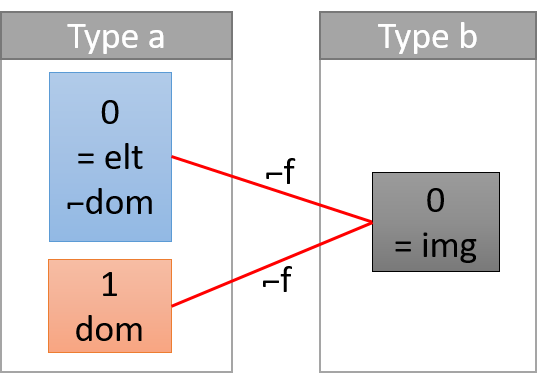
\includegraphics[width=8cm]{NonMonotonicExCounterexample}
    \end{minipage} \hfill
    \begin{minipage}{0.45\textwidth}
        Domain for \(a\): \(\{a_0,a_1\}\)\\
        Domain for \(b\): \(\{b_0\}\)\\
        Constraints on valuations:\\
        \(elt = a_0\)\\
        \(\neg dom(a_0)\)\\
        \(dom(a_1)\)\\
        \(img = b_0\)\\
        \(\neg f(a_0,b_0)\)\\
        \(\neg f(a_1,b_0)\)\\
        Execution: change_elt(\(a_1\))
    \end{minipage}\\

    This state satisfies the conjecture because we have \(\neg dom(elt)\), but after executing change_elt(\(a_1\)) the conjecture will be broken.
    Applying the method described in the previous section will give the following invariant:
    \(\forall A:a. \neg(\neg dom(elt) \land dom(A) \land A \neq elt \land \neg f(elt,res) \land \neg f(A,res))\)

    However, this invariant is not correct. For instance, the following state doesn't satisfy it and can be obtained through a valid execution:

    \begin{minipage}{0.45\textwidth}
        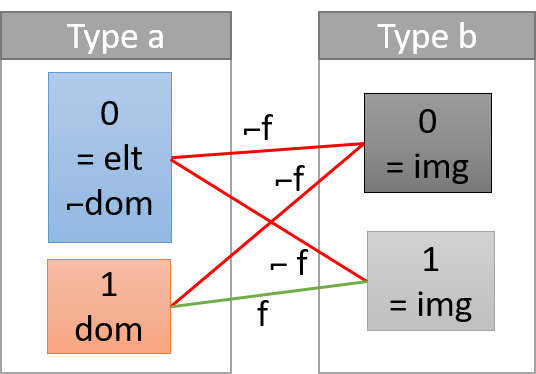
\includegraphics[width=8cm]{NonMonotonicExValid}
    \end{minipage} \hfill
    \begin{minipage}{0.45\textwidth}
        One element \(b_1\) has been added to \(b\)\\
        with the following new valuations:\\
        \(\neg f(a_0,b_1)\)\\
        \(f(a_1,b_1)\)\\
        This time, the conjecture remains satisfied after executing any action.\\
        In particular, executing change_elt(\(a_1\)) will not break the conjecture anymore.
    \end{minipage}\\

    Indeed, the course of the execution of change_elt(\(a_1\)) can be altered just by adding a new element to \(b\)
    (without changing anything else). In this example, it is due to the use of the \textit{if some} statement.
    More generally, it can be caused by non-determinism, by the use of quantified formulas, or anything that explores all the elements of a sort.

    \begin{definition}[Monotonicity]
        A statement \(s\) is monotonic iff, for any two states \(S_1\) and \(S_2\) such that \(S_1 \sqsubseteq S_2\)
        (\(S_1\) is a substructure of \(S_2\)), any states \(S_1'\) and \(S_2'\) that can respectively be obtained after executing
        \(s\) on \(S_1\) and \(S_2\) are such that \(S_1' \sqsubseteq S_2'\).

        An invariant \(P\) is monotonic iff, for any two states \(S_1\) and \(S_2\) such that \(S_1 \sqsubseteq S_2\),
        if \(S_1\) \textbf{doesn't} satisfy \(P\) then \(S_2\) doesn't satisfy \(P\).
    \end{definition}

    \begin{property}
        For a counterexample \((S,E)\), if \(E\) is monotonic \textbf{and} the broken invariant is monotonic (and correct),
        then there exists a correct universal invariant that is not satisfied by \(S\) (we say that the invariant `captures' the counterexample).
    \end{property}
    \begin{property}
        If there exists a correct universal invariant that is not satisfied by \(S\), then
        the naive counterexample generalization method will always generate such an invariant.
        More precisely, it will generate the weakest universal invariant that is not satisfied by \(S\).

        If there is no such invariant, the invariant generated will be incorrect.
    \end{property}
    
    A proof for this last property can be found in this\cite{Karbyshev:2017:PIU:3065931.3022187} article (lemma 1).

    \section{Improving the result with symbolic bounded verification}

    Symbolic bounded verification is a method to check whether a formula is a k-invariant or not:

    \begin{definition}[k-invariant]
        A formula is a k-invariant if it is satisfied after any valid execution of k steps or less
        (that is, any execution of the init action followed by at most k other actions).
    \end{definition}
    
    In order to check whether a formula \(Q\) is a k-invariant or not, we can check the validity of the following formula:

    \( A \Rightarrow \bigwedge\limits_{j=0}^k wp(\text{init}; (\text{action}_1|\ldots|\text{action}_n)^j, Q) \)\\
    where \(A\) refers to the axioms and `\(\text{statement}^j\)' is the sequential composition of \(j\) copies of `statement'.

    In order to check the validity of this formula (for a given \(k\)), we can just check the satisfiability of its negation.
    According to the section 1.4, it is decidable (for \(A\) of the form \(\exists^*\forall^*\) and \(Q\) of the form \(\forall^*\exists^*\)).
    Note that symbolic bounded verification does not allow us to find k-invariants, it can only be used to check whether a formula is a k-invariant or not.

    The naive counterexample generalization method can be improved by using symbolic bounded verification\cite{Padon:2016:ISV:2908080.2908118}:
    \begin{itemize}
        \item It could allow us to know when a generated invariant is not correct.
        Actually, we cannot be sure that an invariant is correct using this method (because it does not analyze executions of length \(> k\)),
        but in practice taking \(k=5\) is sufficient to detect incorrect invariants almost everytime.
        \item It allows us to generate simpler and more general invariants. Indeed, instead of generating a formula that
        aggregates all constraints of \(constr(S)\), we are able to only keep a minimal number of constraints
        such that the resulting invariant is still correct. It can be done quite efficiently by computing a minimal unSAT core using a SMT-solver.
        \item If the program that we want to check is not correct (it doesn't match the specifications), symbolic bounded verification
        can sometimes allow us to find it out, while a naive counterexample generalization would just generate incorrect invariants.
    \end{itemize}\hfill

    \textbf{Reliability}: This method can generate an incorrect invariant if the boundary \(k\) for the symbolic bounded verification
    is too small (sometimes we can't go beyond \(k=3\) in a reasonable time). This method can only generate universal invariants,
    so it will fail if there is no universal invariant that can capture the counterexample (case of non-monotonicity, see section 2.4).\\

    \textbf{Decidability}: All invariants generated are universal, so it never causes any decidability issue.\\

    \textbf{Efficiency}: Invariants generated are quite small and simple. They are more focused than weakest preconditions
    (because they are issued from one precise counterexample) so they can be understood more easily.
    They do not contain any useless litteral, so we can expect them to be quite strong.\\

    This method seems less reliable than just computing the weakest precondition, however it generates invariants that are much more interesting.
    This is the method that is currently implemented by IVy in order to help the user to synthesize inductive invariants interactively.

\chapter{Contributions}

    \section{Course of my internship}

    I spent the first half of my 5-months internship to study the differents aspects of IVy. I wrote some basic protocols in order to get
    familiar with it, I read many articles in order to be aware of the state-of-the-art, etc.

    Finally, I decided to work on the invariant synthesis, and more specifically the counterexample generalization:
    \begin{itemize}
        \item I have proposed a new method to select the important constraints of the counterexample, based on an analysis of the execution of the counterexample.
        This approach is quite complementary with the current IVy approach (symbolic bounded verification): both approaches can be combined. 
        \item I have extended this method with an additional process that can generate correct invariants of the form \(\forall^*\exists^*\)
        when no correct universal invariant exists.
        \item I have implemented a proof of concept for these methods, using the languages F\# and OCaml and the SMT-Solver Z3\cite{z3ref}.        
        \item I have analyzed and compared the guarantees of all these different approaches.
    \end{itemize}

    \section{Filtering constraints by analyzing the execution}

    The problem we want to solve is as follows: given a counterexample (\(S,E\)) (\(S\) being the initial state and \(E\) a deterministic statement describing the execution of an action),
    we want to highlight a subset of \(constr(S)\) (see section 2.3) as small as possible, such that there is no valid state (= state that can be reached after a valid run) that can satisfy these constraints
    (for non-monotonic counterexamples it is not always possible, but this case will be treated in section 3.3).

    To solve this problem, the IVy approach is to use symbolic bounded verification (see section 2.5) to minimize the number of constraints (the problem is encoded as an unSAT core that can be minimized by a SMT-solver).
    My approach is very different:
    \begin{enumerate}
        \item We compute \(S'\) the state obtained after the execution of \(E\) from \(S\).
        \item We try to compute a subset \(C'\) of \(constr(S')\) (as small as possible) such that all states satisfying \(C'\) (modulo renaming of the concrete values)
        evaluate the current invariant to the same value (here, to false). More precisely, we compute a set of `marks', a `mark' being a pointer to an important constraint:
        it can have the form \(symbol(concrete\_value_1,\ldots,concrete\_value_n)\) or \(concrete\_value_1 \neq concrete\_value_2\).
        \item We retropopagate these marks through the execution of \(E\) in order to obtain a subset \(C\) of \(constr(S)\) such that
        all states satisfying \(C\) (modulo renaming of the concrete values) can reproduce the execution \(E\) and satisfy \(C'\) at the end (and so, break the invariant).
    \end{enumerate}

    To perform the step 2, we can use the following algorithm (formulas and terms are assimilated):

    \begin{algorithm}[H]
        \SetKwFunction{MFV}{Compute_marks}%
        \SetKwProg{Fn}{Function}{}{end}
        \SetKwSwitch{Match}{Case}{Other}{match}{}{case}{otherwise}{endcase}{end}
        \Fn{\MFV{S,V}}{
            \KwData{a state \(S\), a formula or a term \(V\)}
            \KwResult{a set of marks \(M\) that points to some important constraints in \(constr(S)\)}

            \Match{V}{
                \uCase{symbol(\(t_1,\ldots,t_n\))}{
                    Compute \(M_1,\ldots,M_n\) the marks for \(t_1,\ldots,t_n\)\;
                    Compute \(v_1,\ldots,v_n\) the evaluation of \(t_1,\ldots,t_n\) in \(S\)\;
                    \KwRet{\(\{symbol(v_1,\ldots,v_n)\} \cup \bigcup M_k\)}\;
                }
                \uCase{\(t_1 = t_2\)}{
                    Compute \(v_1,v_2\) the evaluation of \(t_1,t_2\) in \(S\)\;
                    \uIf {\(v_1 = v_2\)} {
                        \KwRet{\MFV{\(S,t_1\)} \(\cup\) \MFV{\(S,t_2\)}}\;
                    }
                    \uElse {
                        \KwRet{\MFV{\(S,t_1\)} \(\cup\) \MFV{\(S,t_2\)} \(\cup\ \{v_1 \neq v_2\}\)}\;
                    }
                }
                \uCase{\(\neg F\)}{
                    \KwRet{\MFV{\(S,F\)}}\;
                }
                \uCase{\(F_1 \lor F_2\)}{
                    Compute \(b_1,b_2\) the evaluation of \(F_1,F_2\) in \(S\)\;
                    \uIf {\(b_1\)} {
                        \KwRet{\MFV{\(S,F_1\)}}\;
                    }
                    \uElseIf{\(b_2\)}{
                        \KwRet{\MFV{\(S,F_2\)}}\;
                    }
                    \uElse {
                        \KwRet{\MFV{\(S,F_1\)} \(\cup\) \MFV{\(S,F_2\)}}\;
                    }
                }
                \uCase{\(\forall x:a. F(x)\)}{
                    \uIf {there exists \(x_f \in a\) such that \(F(x_f)\) evaluates to false} {
                        \KwRet{\MFV{\(S,F(x_f)\)}}\;
                    }
                    \uElse {
                        \tcc{potential non-monotonicity, see section 3.3}
                        \KwRet{\(\bigcup_{x_t \in a}\) \MFV{\(S,F(x_t)\)}}
                    }
                }
                \uCase{\(\ldots\)}{}
            }
        }
        %\caption{Computing marks for a term or a formula}
    \end{algorithm}\hfill

    For instance, at the end of the counterexample of the section 2.4,
    the formula \(dom(elt) \rightarrow f(elt,img)\) is not satisfied and the marked constraints would be:\\
    \( \{ elt=a_1\ ;\ dom(a_1)=true\ ;\ img=b_0\ ;\ f(a_1,b_0)=false \} \)

    To perform the step 3, we can use the following algorithm:

    \begin{algorithm}[H]
        \SetKwFunction{MFV}{Compute_marks}%
        \SetKwFunction{RPM}{Retropopagate}%
        \SetKwProg{Fn}{Function}{}{end}
        \SetKwSwitch{Match}{Case}{Other}{match}{}{case}{otherwise}{endcase}{end}
        \Fn{\RPM{M',E,S}}{
            \KwData{a set of marks \(M'\) computed after the execution of the deterministic statement \(E\) from the state \(S\)}
            \KwResult{a new set of marks \(M\) that points to some important constraints in \(constr(S)\)}

            \Match{E}{
                \uCase{skip}{\KwRet{\(M'\)}\;}
                \uCase{\textbf{f}(\(\bar{x}\)) := \( t(\bar{x}) \)}{
                    \(M \leftarrow M'\)\;
                    \For{$\bar{x_0}$ such that \textbf{f}(\(\bar{x_0}\)) \(\in M\)}{
                        \(M \leftarrow (M\backslash\{\)\textbf{f}(\(\bar{x_0}\))\(\}) \cup \MFV(S,t(\bar{x_0}))\)\;
                    }
                    \KwRet{\(M\)}\;
                }
                \uCase{assume \( \phi_{EA} \)}{
                    \KwRet{\(M' \cup \MFV(S,\phi_{EA})\)}\;
                }
                \uCase{\( E_1 \) ; \( E_2 \)}{
                    Compute \(S'\) the state obtained after executing \( E_1 \) from \( S \)\;
                    \KwRet{\(\RPM(\RPM(M',E_2,S'),E_1,S)\)}\;
                }
            }
        }
        %\caption{Retropropagate marks through the execution of a statement}
    \end{algorithm}\hfill

    For instance, after having applied this algorithm to the example of the section 2.4 (all primitives used in this example can be translated to RML),
    we can detect that the execution is not monotonic, and we obtain the following marked constraints:\\
    \(\{img=b_0 ; dom(a_1) ; \neg f(a_1,b_0)\} \quad \longrightarrow \quad \forall A:a.\ \neg (dom(A) \land \neg f(A,img))\)\\
    Note that this invariant is much simpler than the one produced by keeping all the constraints (naive generalization, see section 2.3), but it is still incorrect.\\

    This approach has some advantages compared to the current IVy method:
    \begin{itemize}
        \item It doesn't need to use symbolic bounded verification, which can return an incorrect output if \(k\) is too small (and it can take too much time for bigger \(k\)).
        \item It can detect potential non-monotonicity in the code.
        \item For a non-monotonic counterexample, it can still gather some important constraints, even if there is no correct universal invariant that can capture the counterexample.
        From these constraints, a correct invariant of the form \(\forall^*\exists^*\) can sometimes be generated, as we will see in the section 3.3.
    \end{itemize}

    The major drawback is that, sometimes, some useless constraints are not eliminated (because the computation of the marks is not optimal).
    As a consequence, resulting invariants can be more complicated and weaker than invariants generated using symbolic bounded verification.
    However, the two approaches can be used together: symbolic bounded verification can be used after having already filtered the constraints with this method.
    In this way, the advantages of the two methods are combinated. Moreover, the unSAT core to minimize will be smaller, so it will be done faster.

    \section{Case of non-monotonicity}

    As we have seen in section 2.4, some non-monotonic counterexamples can't be captured by any correct universal invariant.
    For this reason, if some potential non-monotonicity is detected during the computation of marks,
    a second process is performed in order to know whether the generated conjecture is correct or not, and to fix it if it is not correct.
    
    In order to do that, we can try to find some valid states that satisfy all the constraints \(C\).
    Such states would be the witnesses of the non-correctness of the universal invariant generated.
    Moreover, if we find such a state, we can use it to weaken the generated conjecture.
    Otherwise, we know that the universal invariant generated is already correct.
    In this section, we will see how to find such states, and in the next section we will see how to use them to weaken the conjecture.

    Let \((S,E)\) be the initial counterexample, let \(C\) be the constraints of \(S\) that have been marked.
    We want to find a state \(S_v\) such that:
    \begin{enumerate}
        \item \(S_v\) satisfies all the constraints \(C\). It implies that the domains of \(S_v\) contain all concrete values that appear in \(C\).
        However, the domains of \(S_v\) can also contain some other elements.
        \item \(S_v\) is a valid state (it can be reached after a valid run).
    \end{enumerate}

    The first condition is easy to express with a formula, but the second condition is more complicated (it would probably need some model checking).
    However, we can approximate it with this other condition (which is weaker, if we assume that the current invariant is correct):
    \(S_v\) satisfies the current invariant and the axioms, and doesn't break any of them after one step (in particular after executing the action that is executed in the counterexample).
    We can express this new condition with the following formula:

    \(A \land I \land wp(\text{action}_1|\ldots|\text{action}_n,I)\)

    Note that checking the satisfiability of this formula is not always decidable (so it may not terminate), because the weakest precondition is not always EPR (see section 2.2).
    However, it was not an issue for the examples that I have tested.

    If the conditions 1 and 2 are satisfiable, we can compute a finite model: it gives us a state \(S_v\) as desired.
    We will see in the next section how to produce a formula \(F_v\) that `generalizes' this state and use it to weaken the generated invariant.
    By adding as a third condition the negation of \(F_v\), an other valid state can be searched.
    This process can potentially not terminate if a new valid state is always found. Indeed, it could be compared to the whole process of finding an inductive invariant:
    \begin{itemize}
        \item To find an inductive invariant, we start from the safety properties and we sthrengthen them until there are no more counterexamples.
        \item To generate a valid invariant from a non-monotonic counterexample, we first generate an universal invariant and we weaken it until there are no more valid states satisfying it.
    \end{itemize}
    However, this process of weakening is much more likely to terminate than the whole process of finding an inductive invariant, because the search space is more restricted:
    we are only looking for valid states that satisfy the constraints \(C\).

    \section{Weakening the conjecture}

    Once we have a valid state \(S_v\) that satisfies all the marked constraints \(C\) of the counterexample,
    we will generalize it and we will build a new invariant that will allow valid states that are similar to \(S_v\).

    The process of generalization of \(S_v\) is quite similar to the process of generalization of the counterexample \((S,E)\).
    First, we can compute a subset \(C_v\) of \(constr(S_v)\) by computing marks for some relevant executions starting in \(S_v\)
    (it will not be detailled here, but the idea is to find an execution that is as close to \(E\) as possible).
    Note that symbolic bounded verification can't be used here: we don't want our formula to be a k-invariant (= to be satisfied by all valid k-executions),
    but only to be satisfied by at least one valid execution.
    Then, we remove from \(C_v\) every constraint that is already in \(C\) in order to keep only constraints that are specific to \(S_v\).

    Next, we replace each different concrete value in \(C_v\) by a fresh existentially quantified variable, but only for concrete values that are specific to \(S_v\):
    concrete values that also appear in \(C\) are kept as they are.
    This will give us a semi-generalized formula \(F_v\) that characterize, among the states satisfying \(C\), those that also
    contains a substructure isomorphic to \(S_v\). Note that it may exist some states that satisfy \(F_v\) but that are not
    valid (again, due to a potential non-monotonicity of the negation of the current invariant).
    However, it is not a major issue since it will not compromise the correctness of the invariant that will be generated.

    Now, we can build a new invariant that will not exclude states similar to \(S_v\).
    We still want to focus on states that satisfy \(C\), but since we only want to characterize invalid states, we don't want to include states that satisfy \(F_v\).
    Thus, we use the following formula: \( C \land (\neg F_v) \).
    This formula still contains concrete values (those that appear in \(C\)), so we must replace them by existentially quantified variables.
    The resulting formula has the form \( \exists^* \ldots \land \neg(\exists^* \ldots) \). After negating it, we obtain a new invariant of the form
    \( \forall^* \ldots \rightarrow (\exists^* \ldots) \), that is an invariant with a \(\forall^*\exists^*\) prefix.

    Here is a table that illustrates this process on the example of the section 2.4:\\
    \begin{tabular}{|l|c|c|}
        \hline
        & Counterexample \((S,E)\) & Valid state \(S_v\) \\
        \hline
        Shared concrete constraints & \multicolumn{2}{c|}{\(dom(a_1)\)}\\
        (after reduction and simplification) & \multicolumn{2}{c|}{\(\neg f(a_1,img)\)}\\
        \hline
        Shared concrete values & \multicolumn{2}{c|}{\(\{ a_1 \}\)} \\
        \hline
        Constraints specific to \(S_v\) (after reduction) & - & \(f(a_1,b_1)\) \\
        \hline
        Concrete values specific to \(S_v\) & - & \(\{b_1\}\) \\
        \hline
        Semi-generalized formula \(F_v\) & - & \(\exists B:b.\ f(a_1, B)\) \\
        \hline
        New generated invariant & \multicolumn{2}{c|}{\(\forall A:a.\ dom(A) \land \neg f(A,img) \rightarrow \exists B:b.\ f(A,B) \)}\\
        \hline
    \end{tabular}\\

    \section{Comparison with other methods}

    Let's evaluate the method presented in this chapter using the same criteria as before.

    \textbf{Reliability}: If we assume that the initial invariant is correct, then this algorithm always generate correct invariants.
    However, if there is no correct universal invariant that can capture the counterexample, this algorithm might not terminate (see section 3.3).\\

    \textbf{Decidability}: If there exists a correct universal invariant that can capture the counterexample, then such an invariant will be produced.
    Otherwise, an invariant of the form \(\forall^*\exists^*\) will be produced. It may cause some decidability issues that the user will have to solve
    (it is challenge that the user will often have to face when using IVy, see section 1.5).\\

    \textbf{Efficiency}: Invariants generated are quite small and simple because they only contains elements that have played an important role in the execution of the counterexample.
    Symbolic bounded verification can be used to improve the result.\\

    Here is a table that compare the different methods of invariant synthesis:\\
    \begin{tabularx}{\textwidth}{|l|X|X|X|}
        \hline
            & Weakest precondition & \multicolumn{2}{c|}{Counterexample generalization}\\
        \cline{3-4}
            & (section 2.2) & Symbolic bounded verification (section 2.5) & Execution analysis + Weakening (chapter 3)\\
        \hline
            Reliability & \textcolor{ForestGreen}{Always terminate, always correct} &
            \textcolor{Red}{Can only generate universal invariants (no guarantee for non-monotonic counterexamples), incorrect if \(k\) is too small}
            & \textcolor{Dandelion}{Can generate universal invariants when possible, otherwise can generate \(\forall^*\exists^*\) invariants (but may not terminate in this case)}\\
        \hline
            Decidability & \textcolor{Dandelion}{Not always EPR. Additional restrictions can be imposed to always have EPR weakest preconditions}
            & \textcolor{ForestGreen}{Generated invariants are always universal (so they always can be checked in a decidable way)}
            & \textcolor{ForestGreen}{Generated invariants are universal when possible (in particular, for monotonic counterexamples)}\\
        \hline
            Efficiency & \textcolor{Red}{Generated invariants are very long, unreadable, and often too weak}
            & \textcolor{ForestGreen}{Generated invariants are simple and don't contain any useless litteral}
            & \textcolor{ForestGreen}{Generated invariants are quite simple, symbolic bounded verification can be used to improve the result}\\
        \hline
    \end{tabularx}\\

    \section{Conclusion}

    This internship has been a very fulfulling experience for me. I have experimented an aspect of research
    that I had not experienced during my last year's internship:
    during the first half of the internship, I had to read articles and to experiment in order to find ideas.
    My comprehension of the subject has really evolved during this time.
    I explored many different problematics before focusing on the invariant synthesis.
    For instance, one of my attempts was to try to add some more advanced typing to IVy, without loosing decidability.
    In particular, I have studied \textit{session types} (it was even more interesting since there is a lot of session types experts in Carnegie Mellon University).
    Finally, I gave up this idea since the linearity of session types seemed hardly reconciliable with the distributed and decentralized aspects of the protocols
    that we wanted to prove.

\bibliographystyle{unsrt}
\bibliography{sample}

\appendix 
\chapter{Experimental results}
%The complexity of the different operations has not been treated in this report.
%Indeed, checking the satisfiability of EPR formulas is NEXPTIME-complete.
%However, studying the worst case complexity is not very relevant here since it would be very different
%from the complexity observed experimentaly.

    \section{A queue}

    Here is an implementation and a specification of a queue.
    The initial safety properties are the two first conjectures (free capital variables are quantified universally by default).\\\\
    \includegraphics[width=17cm]{Queue1}\\
    \includegraphics[width=17cm]{Queue2}\\

    The four last conjectures have been found using my proof of concept (without any modification from the user).
    The combination of all these invariants is inductive.

    As we can see, one of these invariants has a \(\forall^*\exists^*\) prefix: it would not have been found using the current invariant synthesis tool of IVy.
    We can also notice that the second invariant that has been found is strictly weaker than the third (it can be removed).
    It is due to the fact that the second counterexample found was too specific: its structure has imposed some (useless) equality constraints.
    However, generating the associated invariant and adding it to the set has permitted to find an other more general counterexample (the third).
\end{document}

